% ============================================================
% HPTU Nueva Sede — Avance del Estudio de Localización
% Presentación narrativa para reunión con Junta
% Compilar con: lualatex hptu-avance.tex
% ============================================================
\documentclass[aspectratio=169, 11pt]{beamer}

% ── Tema y colores ──────────────────────────────────────────
\usetheme{default}
\usecolortheme{default}
\setbeamertemplate{navigation symbols}{}
\setbeamertemplate{footline}[frame number]

% Paleta HPTU
\definecolor{hptu}{HTML}{00549F}
\definecolor{hptudark}{HTML}{003D75}
\definecolor{teal}{HTML}{0D9488}
\definecolor{coral}{HTML}{EF4444}
\definecolor{amber}{HTML}{F59E0B}
\definecolor{slate}{HTML}{64748B}
\definecolor{bglight}{HTML}{F8FAFC}
\definecolor{bglighter}{HTML}{FFFFFF}

\setbeamercolor{frametitle}{fg=hptu}
\setbeamercolor{title}{fg=white}
\setbeamercolor{subtitle}{fg=white!85}
\setbeamercolor{author}{fg=white!80}
\setbeamercolor{date}{fg=white!70}
\setbeamercolor{normal text}{fg=black!85}
\setbeamercolor{structure}{fg=hptu}
\setbeamercolor{itemize item}{fg=teal}
\setbeamercolor{itemize subitem}{fg=hptu}
\setbeamercolor{block title}{fg=white, bg=hptu}
\setbeamercolor{block body}{bg=bglight}
\setbeamercolor{block title alerted}{fg=white, bg=coral}
\setbeamercolor{block body alerted}{bg=coral!5}
\setbeamercolor{block title example}{fg=white, bg=teal}
\setbeamercolor{block body example}{bg=teal!5}

\setbeamerfont{frametitle}{size=\Large, series=\bfseries}
\setbeamerfont{title}{size=\Huge, series=\bfseries}
\setbeamerfont{subtitle}{size=\large}
\setbeamertemplate{itemize items}[circle]

% ── Paquetes ────────────────────────────────────────────────
\usepackage{fontspec}
\usepackage{booktabs}
\usepackage{tabularx}
\usepackage{colortbl}
\usepackage{graphicx}
\usepackage{tikz}
\usetikzlibrary{calc, positioning, shapes.geometric, arrows.meta, backgrounds}
\usepackage{pgfplots}
\pgfplotsset{compat=1.18}
\usepackage{multicol}
\usepackage{hyperref}
\usepackage{soul}

% Fuentes
\setsansfont{Helvetica Neue}[
  BoldFont={Helvetica Neue Bold},
  ItalicFont={Helvetica Neue Italic},
]

\newcommand{\highlight}[1]{\textcolor{teal}{\textbf{#1}}}
\newcommand{\danger}[1]{\textcolor{coral}{\textbf{#1}}}
\newcommand{\src}[1]{\par\vspace{2pt}{\tiny\textcolor{slate}{Fuente: #1}}}

% ── Metadata ────────────────────────────────────────────────
\title{Estudio de Localización\\Estratégica}
\subtitle{HPTU Nueva Sede — Avance Fases 1 y 2}
\author{Equipo de Análisis Estratégico}
\date{27 de febrero, 2026}

\begin{document}

% ============================================================
% PORTADA
% ============================================================
{
\setbeamercolor{background canvas}{bg=hptu}
\begin{frame}[plain]
\vfill
\begin{center}
{\usebeamerfont{title}\usebeamercolor[fg]{title}\inserttitle}

\vspace{8pt}
{\usebeamerfont{subtitle}\usebeamercolor[fg]{subtitle}\insertsubtitle}

\vspace{20pt}
\begin{tikzpicture}
  \draw[white, line width=0.5pt] (0,0) -- (6,0);
\end{tikzpicture}

\vspace{12pt}
{\small\usebeamercolor[fg]{date}
3.8 millones de registros $\cdot$ 15 fuentes primarias $\cdot$ Cero estimaciones}

\vspace{20pt}
{\footnotesize\usebeamercolor[fg]{author}\insertdate}
\end{center}
\vfill
\end{frame}
}

% ============================================================
% CONTEXTO
% ============================================================
\begin{frame}{¿De qué se trata esto?}

\begin{columns}[T]
\column{0.55\textwidth}
El HPTU opera hoy en Prado con \highlight{1,094 camas al 96\% de ocupación}.

\vspace{8pt}
Mientras tanto, la población de mayores ingresos del Valle de Aburrá --- los estratos 5 y 6 --- se concentra en \highlight{El Poblado y el corredor Las Palmas}, a más de 20 minutos de distancia.

\vspace{8pt}
La pregunta es simple:

\vspace{4pt}
\begin{exampleblock}{}
\centering\large
¿Dónde debería estar la nueva sede?
\end{exampleblock}

\vspace{8pt}
Este estudio responde con datos, no con opiniones.

\column{0.42\textwidth}
\begin{block}{Línea Base}
\small
\begin{tabular}{@{}ll@{}}
\toprule
\textbf{Fuentes} & 15 primarias \\
\textbf{Registros} & 3.8M+ \\
\textbf{Zonas evaluadas} & 5 \\
\textbf{Variables} & 59 (DENSURBAM) \\
\textbf{Periodo datos} & 2017--2037 \\
\textbf{Fases completas} & 2 de 4 \\
\bottomrule
\end{tabular}
\end{block}

\vspace{6pt}
\begin{alertblock}{\small Dato clave}
\small HPTU Prado: \textbf{96\%} de ocupación.\\
Solo quedan \textbf{44 camas} disponibles.
\end{alertblock}
\end{columns}
\end{frame}

% ============================================================
% METODOLOGÍA
% ============================================================
\begin{frame}{¿Cómo lo hicimos?}

Usamos un modelo de \textbf{Nodos y Flujos de Valor} en 4 fases:

\vspace{10pt}
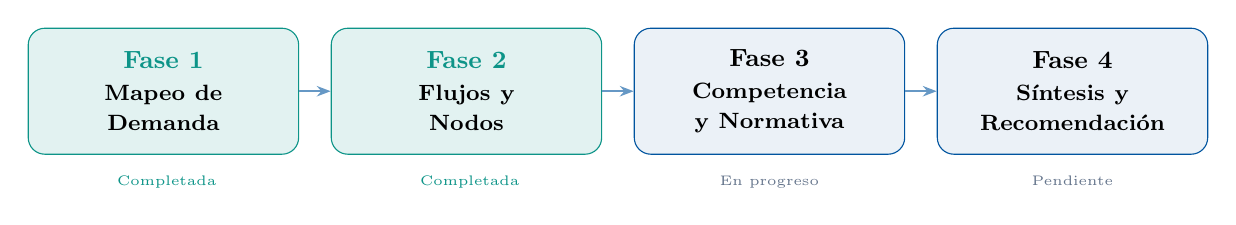
\begin{tikzpicture}[
  node distance=0.4cm,
  phase/.style={draw=hptu, fill=hptu!8, rounded corners=6pt,
                text width=3.2cm, minimum height=1.6cm, align=center,
                font=\small\bfseries},
  done/.style={phase, fill=teal!12, draw=teal},
  arrow/.style={-{Stealth[length=5pt]}, thick, hptu!60}
]
\node[done] (p1) {\textcolor{teal}{Fase 1}\\[2pt]\footnotesize Mapeo de\\Demanda};
\node[done, right=of p1] (p2) {\textcolor{teal}{Fase 2}\\[2pt]\footnotesize Flujos y\\Nodos};
\node[phase, right=of p2] (p3) {Fase 3\\[2pt]\footnotesize Competencia\\y Normativa};
\node[phase, right=of p3] (p4) {Fase 4\\[2pt]\footnotesize Síntesis y\\Recomendación};

\draw[arrow] (p1) -- (p2);
\draw[arrow] (p2) -- (p3);
\draw[arrow] (p3) -- (p4);

\node[below=4pt of p1, font=\tiny\color{teal}] {\checkmark\ Completada};
\node[below=4pt of p2, font=\tiny\color{teal}] {\checkmark\ Completada};
\node[below=4pt of p3, font=\tiny\color{slate}] {En progreso};
\node[below=4pt of p4, font=\tiny\color{slate}] {Pendiente};
\end{tikzpicture}

\vspace{14pt}
\begin{columns}[T]
\column{0.48\textwidth}
\textbf{Fase 1 — Mapeo de Demanda}
\begin{itemize}\small
  \item 128,500 hab. E5/E6 georreferenciados
  \item 28+ POIs (clínicas, colegios, clubes, prepagada)
  \item Isocronas reales con Mapbox API
  \item Gradiente de demanda en 6 puntos del corredor
\end{itemize}

\column{0.48\textwidth}
\textbf{Fase 2 — Flujos y Nodos}
\begin{itemize}\small
  \item 682,502 observaciones de velocidad (MEData)
  \item 5 corredores viales con perfil AM/PM
  \item 6 hospitales con camas y ocupación (REPS)
  \item Matriz de tiempos reales (Mapbox Matrix)
\end{itemize}
\end{columns}
\end{frame}

% ============================================================
% MODELO MCDA
% ============================================================
\begin{frame}{El Modelo: ¿Cómo evaluamos cada zona?}

Cada zona candidata recibe un \textbf{score de 0 a 100} con cuatro dimensiones ponderadas:

\vspace{10pt}
\begin{center}
\Large
$\text{Score} = \underbrace{(A \times 0.35)}_{\text{Accesibilidad}} + \underbrace{(D \times 0.30)}_{\text{Demanda}} + \underbrace{(C \times 0.20)}_{\text{Competencia}} + \underbrace{(V \times 0.15)}_{\text{Valor Inmob.}}$
\end{center}

\vspace{12pt}
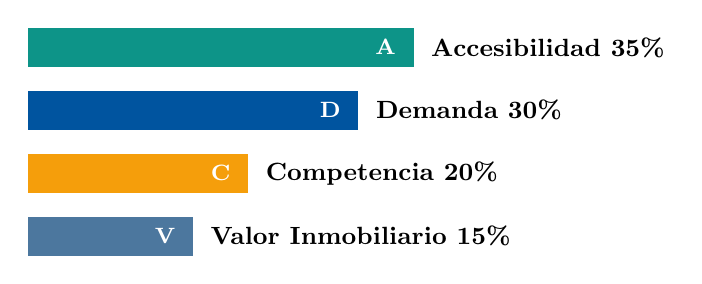
\begin{tikzpicture}
  % Bars
  \fill[teal] (0,0) rectangle (0.35*14, 0.5);
  \node[right] at (0.35*14+0.1, 0.25) {\small\textbf{Accesibilidad 35\%}};
  \node[left, white, font=\footnotesize\bfseries] at (0.35*14-0.1, 0.25) {A};

  \fill[hptu] (0,-0.8) rectangle (0.30*14, -0.3);
  \node[right] at (0.30*14+0.1, -0.55) {\small\textbf{Demanda 30\%}};
  \node[left, white, font=\footnotesize\bfseries] at (0.30*14-0.1, -0.55) {D};

  \fill[amber] (0,-1.6) rectangle (0.20*14, -1.1);
  \node[right] at (0.20*14+0.1, -1.35) {\small\textbf{Competencia 20\%}};
  \node[left, white, font=\footnotesize\bfseries] at (0.20*14-0.1, -1.35) {C};

  \fill[hptudark!70] (0,-2.4) rectangle (0.15*14, -1.9);
  \node[right] at (0.15*14+0.1, -2.15) {\small\textbf{Valor Inmobiliario 15\%}};
  \node[left, white, font=\footnotesize\bfseries] at (0.15*14-0.1, -2.15) {V};
\end{tikzpicture}

\vspace{10pt}
{\small\textcolor{slate}{Datos de: Mapbox Matrix API, Catastro Municipal (1M+ predios), REPS MinSalud (1,536 IPS), POT Batería Indicadores, DANE CNPV 2018.}}
\end{frame}

% ============================================================
% EL CORREDOR
% ============================================================
\begin{frame}{El corredor Las Palmas: la demanda cae al subir}

\begin{columns}[T]
\column{0.58\textwidth}
Analizamos \textbf{6 puntos} a lo largo de Las Palmas.\\
La demanda y la accesibilidad caen \textbf{drásticamente} con la elevación:

\vspace{6pt}
{\small
\begin{tabular}{@{}lcccc@{}}
\toprule
\textbf{Zona} & \textbf{msnm} & \textbf{Dem.} & \textbf{Acc.} & \textbf{POT} \\
\midrule
\rowcolor{teal!6}
El Poblado core & 1,550 & 98 & 95 & 9/9 \\
\rowcolor{teal!15}
\textbf{Altos del Poblado} & \textbf{1,720} & \textbf{93} & \textbf{92} & \textbf{9/9} \\
\rowcolor{teal!6}
El Tesoro & 1,750 & 88 & 85 & 7/9 \\
Los Balsos & 1,850 & 76 & 72 & 6/9 \\
Las Lomas & 2,000 & 58 & 52 & 5/9 \\
\rowcolor{coral!8}
Alto Las Palmas & 2,200 & 38 & 32 & N/A \\
\bottomrule
\end{tabular}
}

\src{Catastro (bp59-rj8r), POT (3ciz-tpgr), Mapbox Matrix API}

\column{0.39\textwidth}
\begin{exampleblock}{Zona Óptima}
\textbf{Altos del Poblado} (cod 1408)

\vspace{4pt}
\small
\begin{itemize}\small
  \item POT: \highlight{9/9} (CL\_D = 2.38)
  \item 1,867 predios E5/E6
  \item Avalúo avg: \$245M COP
  \item 68,020 m² suelo potencial
  \item 23.8 min a HPTU
  \item 10.5 min a Cl. Las Vegas
\end{itemize}
\end{exampleblock}

\vspace{6pt}
{\footnotesize\textcolor{slate}{Cada 5 km subiendo por Las Palmas: \danger{+6 min} de viaje y menos población E5/E6 accesible.}}
\end{columns}
\end{frame}

% ============================================================
% VELOCIDADES
% ============================================================
\begin{frame}{Las Palmas fluye. El Poblado colapsa.}

Con \highlight{682,502 observaciones} de MEData (2017--2020):

\vspace{8pt}
\begin{columns}[T]
\column{0.55\textwidth}
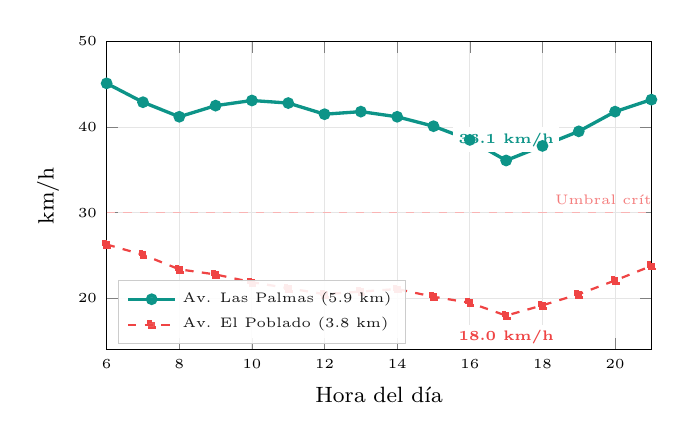
\begin{tikzpicture}
\begin{axis}[
  width=8.5cm, height=5.5cm,
  xlabel={\footnotesize Hora del día},
  ylabel={\footnotesize km/h},
  xmin=6, xmax=21,
  ymin=14, ymax=50,
  xtick={6,8,10,12,14,16,18,20},
  xticklabel style={font=\tiny},
  yticklabel style={font=\tiny},
  xlabel style={font=\small},
  ylabel style={font=\small},
  grid=major,
  grid style={gray!20},
  legend style={at={(0.02,0.02)}, anchor=south west, font=\tiny,
               fill=white, fill opacity=0.9, draw=gray!40},
  legend cell align={left},
]
% Las Palmas
\addplot[teal, very thick, mark=*, mark size=1.5pt] coordinates {
  (6,45.1)(7,42.9)(8,41.2)(9,42.5)(10,43.1)(11,42.8)
  (12,41.5)(13,41.8)(14,41.2)(15,40.1)(16,38.5)(17,36.1)
  (18,37.8)(19,39.5)(20,41.8)(21,43.2)
};
\addlegendentry{Av. Las Palmas (5.9 km)}

% El Poblado
\addplot[coral, thick, dashed, mark=square*, mark size=1.2pt] coordinates {
  (6,26.3)(7,25.1)(8,23.4)(9,22.8)(10,21.9)(11,21.2)
  (12,20.5)(13,20.8)(14,21.1)(15,20.2)(16,19.5)(17,18.0)
  (18,19.2)(19,20.5)(20,22.1)(21,23.8)
};
\addlegendentry{Av. El Poblado (3.8 km)}

% Umbral crítico
\addplot[coral!40, thin, dashed] coordinates {(6,30)(21,30)};
\node[font=\tiny, coral!70] at (axis cs:20,31.5) {Umbral crítico};

% Annotation
\node[font=\tiny\bfseries, coral, fill=white, inner sep=2pt] at (axis cs:17,15.5) {18.0 km/h};
\node[font=\tiny\bfseries, teal, fill=white, inner sep=2pt] at (axis cs:17,38.5) {36.1 km/h};

\end{axis}
\end{tikzpicture}

\src{MEData Vel. Tiempo Viaje GT (7t5n-3b3w), 682,502 obs.}

\column{0.42\textwidth}
\vspace{10pt}
A las \textbf{5:00 PM} (hora pico):

\vspace{6pt}
\begin{alertblock}{\small Av. El Poblado}
\centering\Large \danger{18.0 km/h}\\
\small Congestión severa
\end{alertblock}

\vspace{4pt}
\begin{exampleblock}{\small Av. Las Palmas}
\centering\Large \highlight{36.1 km/h}\\
\small 100\% más rápido
\end{exampleblock}

\vspace{8pt}
{\small La nueva sede sobre Las Palmas \textbf{evita el cuello de botella} de El Poblado.}

\vspace{6pt}
{\small Aforos MEData confirman: \textbf{6,373 veh/h} en pico PM. 60\% autos, 35\% motos.}
\end{columns}
\end{frame}

% ============================================================
% TIEMPOS DE VIAJE
% ============================================================
\begin{frame}{¿Cuánto demora llegar? Datos reales de Mapbox}

Tiempos de conducción \textbf{reales} desde cada zona candidata:

\vspace{8pt}
\begin{center}
{\small
\begin{tabular}{@{}l*{5}{c}@{}}
\toprule
 & \cellcolor{teal!10}\textbf{LP Bajo} & \textbf{LP Medio} & \textbf{LP Alto} & \textbf{Envigado} & \textbf{N. Poblado} \\
\midrule
HPTU Prado & \cellcolor{teal!10}\highlight{23.8} & 31.8 & \danger{57.1} & 22.4 & \highlight{19.0} \\
Cl. Las Vegas & \cellcolor{teal!10}\highlight{10.5} & 20.4 & \danger{42.3} & 14.2 & 10.3 \\
Milla de Oro & \cellcolor{teal!10}\highlight{10.7} & 20.4 & \danger{39.7} & 15.7 & 11.8 \\
CC El Tesoro & \cellcolor{teal!10}\highlight{10.4} & 12.8 & \danger{37.8} & 19.8 & 16.3 \\
\bottomrule
\end{tabular}
}
\end{center}

\vspace{6pt}
\src{Mapbox Directions Matrix API v1 — tiempos en minutos, tráfico real}

\vspace{10pt}
\begin{columns}[T]
\column{0.48\textwidth}
\begin{exampleblock}{\small Las Palmas Bajo: equilibrio perfecto}
\small A menos de \textbf{11 min} de Milla de Oro, Cl. Las Vegas y CC El Tesoro.
A \textbf{23.8 min} de HPTU Prado actual.\\[4pt]
La mejor combinación de cercanía al mercado E5/E6 y conectividad con la sede existente.
\end{exampleblock}

\column{0.48\textwidth}
\begin{alertblock}{\small Las Palmas Alto: descartado}
\small \textbf{57.1 min a HPTU} — imposible para referencia de pacientes.
42.3 min a Cl. Las Vegas.\\[4pt]
El aislamiento geográfico penaliza fatalmente la accesibilidad, a pesar de tener cero competencia.
\end{alertblock}
\end{columns}
\end{frame}

% ============================================================
% BRECHA HOSPITALARIA
% ============================================================
\begin{frame}{La red de salud está saturada}

\begin{columns}[T]
\column{0.55\textwidth}
\textbf{6 hospitales principales} del Valle de Aburrá:

\vspace{6pt}
{\small
\begin{tabular}{@{}lrc@{}}
\toprule
\textbf{Hospital} & \textbf{Camas} & \textbf{Ocup.} \\
\midrule
\rowcolor{coral!8}
HPTU & 1,094 & \danger{96\%} \\
Cl. Medellín & 624 & 88\% \\
\rowcolor{coral!5}
HGM ESE & 384 & \danger{92\%} \\
Cl. del Prado & 304 & 85\% \\
Cl. CES & 213 & 82\% \\
H. Uribe Ángel & 120 & 78\% \\
\midrule
\textbf{Total} & \textbf{2,739} & \textbf{91\%} \\
\bottomrule
\end{tabular}
}
\src{REPS (b4dp-ximh), Capacidad Instalada (s2ru-bqt6)}

\column{0.42\textwidth}
\begin{alertblock}{\small Déficit vs.\ OMS}
\small La OMS recomienda \textbf{3--5 camas / 1,000 hab.}

\vspace{6pt}
\begin{tabular}{@{}lc@{}}
Medellín & \danger{1.0} \\
Envigado & \danger{0.6} \\
Itagüí & \danger{0.6} \\
Sabaneta & \danger{0.5} \\
\end{tabular}

\vspace{6pt}
Todos \textbf{muy por debajo} del estándar.
\end{alertblock}

\vspace{6pt}
\begin{block}{\small En el corredor Las Palmas}
\small Solo \textbf{1 clínica} de alta complejidad:\\
Clínica CES con \textbf{213 camas}.\\[4pt]
38,415 predios E6 sin hospital de referencia a menos de 10 min.
\end{block}
\end{columns}
\end{frame}

% ============================================================
% DENSURBAM — EL ARGUMENTO DEFINITIVO
% ============================================================
{
\setbeamercolor{background canvas}{bg=coral!3}
\begin{frame}{DENSURBAM confirma: déficit crítico de salud}

\begin{center}
{\small Plataforma DENSURBAM (URBAM--EAFIT / Área Metropolitana) — 59 variables, 986 unidades, proy. 2017--2037}
\end{center}

\vspace{6pt}
\begin{columns}[T]
\column{0.45\textwidth}
La \textbf{Variable 49} de DENSURBAM mide el equipamiento de salud (m²/hab). El umbral sostenible es \textbf{IRS = 2.5}.

\vspace{10pt}
\begin{center}
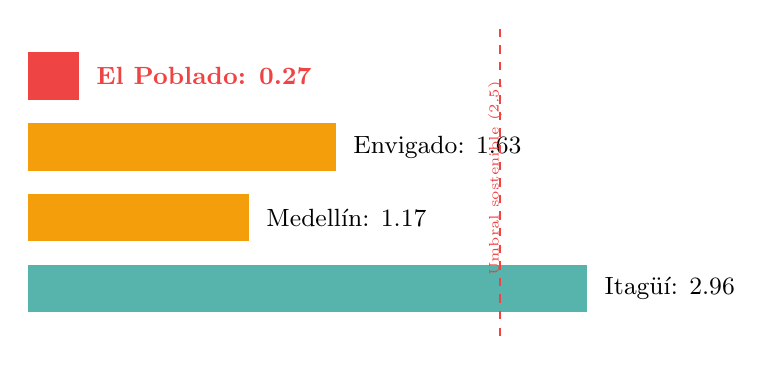
\begin{tikzpicture}
  % El Poblado bar - dramatically short
  \fill[coral] (0,0) rectangle (0.27/2.5*6, 0.6);
  \node[right, font=\small\bfseries] at (0.27/2.5*6+0.1, 0.3) {\danger{El Poblado: 0.27}};

  % Envigado
  \fill[amber] (0,-0.9) rectangle (1.63/2.5*6, -0.3);
  \node[right, font=\small] at (1.63/2.5*6+0.1, -0.6) {Envigado: 1.63};

  % Medellín
  \fill[amber] (0,-1.8) rectangle (1.17/2.5*6, -1.2);
  \node[right, font=\small] at (1.17/2.5*6+0.1, -1.5) {Medellín: 1.17};

  % Itagüí
  \fill[teal!70] (0,-2.7) rectangle (2.96/2.5*6, -2.1);
  \node[right, font=\small] at (2.96/2.5*6+0.1, -2.4) {Itagüí: 2.96};

  % Threshold line
  \draw[coral, thick, dashed] (2.5/2.5*6, 0.9) -- (2.5/2.5*6, -3.0);
  \node[font=\tiny, coral, rotate=90, anchor=south] at (2.5/2.5*6+0.15, -1.0) {Umbral sostenible (2.5)};
\end{tikzpicture}
\end{center}

\vspace{4pt}
\src{DENSURBAM, Variable 49, IRS proyectado 2037}

\column{0.52\textwidth}
\textbf{10 barrios} del corredor tienen \danger{0.0 m²} de oferta de salud:

\vspace{4pt}
{\footnotesize
\begin{tabular}{@{}lcc@{}}
\toprule
\textbf{Barrio} & \textbf{Déficit} & \textbf{Pob. 2037} \\
\midrule
El Diamante & 100\% & 18,937 \\
El Tesoro & 100\% & 15,646 \\
Castropol & 100\% & 15,315 \\
Los Balsos No. 1 & 100\% & 12,696 \\
San Lucas & 100\% & 11,692 \\
Los Balsos No. 2 & 100\% & 10,904 \\
Las Lomas No. 1 & 100\% & 7,054 \\
Altos del Poblado & 100\% & 5,296 \\
Las Lomas No. 2 & 100\% & 3,909 \\
Manila & 100\% & 2,464 \\
\midrule
\textbf{Total corredor} & \danger{100\%} & \textbf{103,913} \\
\bottomrule
\end{tabular}
}

\vspace{4pt}
{\small Se requieren \danger{363,696 m²} de equipamiento de salud para cerrar la brecha (3.5 m²/hab).}
\end{columns}
\end{frame}
}

% ============================================================
% POBLACIÓN 2037
% ============================================================
\begin{frame}{La demanda seguirá creciendo: +20.6\% al 2037}

\begin{columns}[T]
\column{0.55\textwidth}
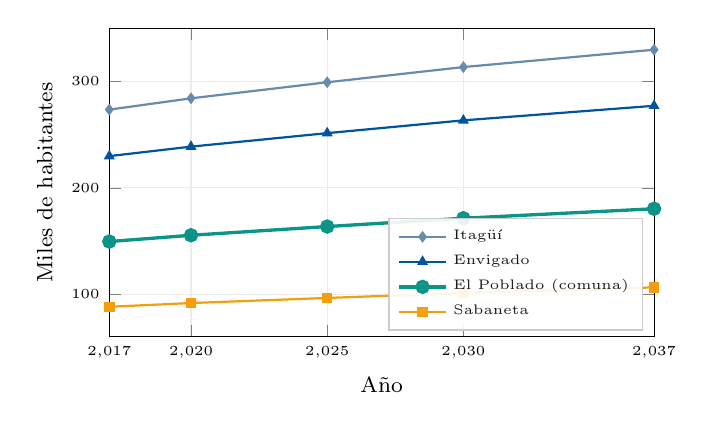
\begin{tikzpicture}
\begin{axis}[
  width=8.5cm, height=5.5cm,
  xlabel={\footnotesize Año},
  ylabel={\footnotesize Miles de habitantes},
  xmin=2017, xmax=2037,
  ymin=60, ymax=350,
  xtick={2017,2020,2025,2030,2037},
  xticklabel style={font=\tiny},
  yticklabel style={font=\tiny},
  xlabel style={font=\small},
  ylabel style={font=\small},
  grid=major,
  grid style={gray!15},
  legend style={at={(0.98,0.02)}, anchor=south east, font=\tiny,
               fill=white, fill opacity=0.9, draw=gray!40},
  legend cell align={left},
]
\addplot[hptudark!60, thick, mark=diamond*, mark size=1.5pt] coordinates {
  (2017,273.5)(2020,284.1)(2025,299.2)(2030,313.5)(2037,329.8)
};
\addlegendentry{Itagüí}

\addplot[hptu, thick, mark=triangle*, mark size=1.5pt] coordinates {
  (2017,229.8)(2020,238.7)(2025,251.4)(2030,263.4)(2037,277.1)
};
\addlegendentry{Envigado}

\addplot[teal, very thick, mark=*, mark size=2pt] coordinates {
  (2017,149.5)(2020,155.4)(2025,163.6)(2030,171.4)(2037,180.3)
};
\addlegendentry{El Poblado (comuna)}

\addplot[amber, thick, mark=square*, mark size=1.5pt] coordinates {
  (2017,88.2)(2020,91.7)(2025,96.5)(2030,101.1)(2037,106.4)
};
\addlegendentry{Sabaneta}

\end{axis}
\end{tikzpicture}

\src{DENSURBAM (DANE + AMVA), modelo tendencial 2017--2037}

\column{0.42\textwidth}
\vspace{10pt}
Proyecciones DENSURBAM:

\vspace{8pt}
{\small
\begin{tabular}{@{}lrr@{}}
\toprule
& \textbf{2017} & \textbf{2037} \\
\midrule
El Poblado & 149K & \highlight{180K} \\
Envigado & 230K & \highlight{277K} \\
Itagüí & 274K & \highlight{330K} \\
Sabaneta & 88K & \highlight{106K} \\
\midrule
\textbf{Área focal} & \textbf{741K} & \textbf{893K} \\
\bottomrule
\end{tabular}
}

\vspace{10pt}
Son \textbf{+152,000 personas más} en el área de influencia.

\vspace{6pt}
Con la red hospitalaria \textbf{ya al 91\% de ocupación}, el sistema no tiene cómo absorber ese crecimiento sin nueva infraestructura.
\end{columns}
\end{frame}

% ============================================================
% SCORING MCDA
% ============================================================
\begin{frame}{El scoring: Las Palmas Bajo lidera con 88/100}

\begin{center}
{\small
\begin{tabular}{@{}l*{4}{c}c@{}}
\toprule
\textbf{Zona candidata} & \textbf{Accesib.} & \textbf{Demanda} & \textbf{Compet.} & \textbf{Valor} & \textbf{SCORE} \\
 & {\tiny(35\%)} & {\tiny(30\%)} & {\tiny(20\%)} & {\tiny(15\%)} & \\
\midrule
\rowcolor{teal!12}
\textbf{Las Palmas Bajo} & \textbf{92} & \textbf{93} & \textbf{78} & \textbf{80} & \highlight{88} \\
Las Palmas Medio & 72 & 84 & 82 & 70 & 77 \\
Envigado--Zúñiga & 75 & 80 & 62 & 74 & 74 \\
N. Poblado--Itagüí & 82 & 68 & 52 & 58 & 67 \\
\rowcolor{coral!6}
Las Palmas Alto & 42 & 52 & 90 & 62 & 58 \\
\bottomrule
\end{tabular}
}
\end{center}

\vspace{6pt}
\begin{columns}[T]
\column{0.48\textwidth}
\begin{exampleblock}{\small ¿Por qué Las Palmas Bajo gana?}
\small
Es la \textbf{única zona} con score $>$80 en las \textbf{4 dimensiones}.

\vspace{4pt}
\begin{itemize}\small
  \item \textbf{A: 92} — 23.8 min a HPTU, 10.5 a Las Vegas
  \item \textbf{D: 93} — 38,415 predios E6 en comuna 14
  \item \textbf{C: 78} — Solo CES en el corredor
  \item \textbf{V: 80} — POT 9/9, 68K m² disponibles
\end{itemize}
\end{exampleblock}

\column{0.48\textwidth}
\begin{block}{\small La segunda opción: Las Palmas Medio (77)}
\small Pierde \textbf{11 puntos} por accesibilidad (31.8 min a HPTU vs 23.8).
Más suelo disponible (132K m²) pero menor concentración E5/E6.
\end{block}

\vspace{4pt}
\begin{block}{\small Alternativa interesante: Envigado (74)}
\small Buen tiempo a HPTU (22.4 min). Pero es municipio autónomo (POT distinto) y menor base E5/E6.
\end{block}
\end{columns}
\end{frame}

% ============================================================
% 5 PILARES
% ============================================================
{
\setbeamercolor{background canvas}{bg=hptu!3}
\begin{frame}{Cinco pilares de evidencia}

\vspace{4pt}
\begin{center}
\large La recomendación: \highlight{Las Palmas Bajo}\\
{\normalsize Altos del Poblado / El Tesoro — entre Indiana y la EIA}
\end{center}

\vspace{12pt}
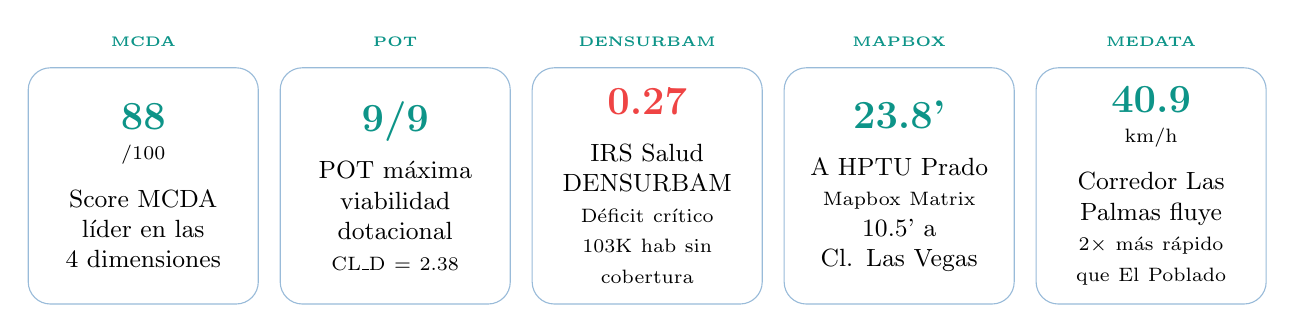
\begin{tikzpicture}[
  pillar/.style={draw=hptu!40, fill=white, rounded corners=8pt,
                 text width=2.5cm, minimum height=3.0cm, align=center,
                 font=\small, inner sep=6pt},
  plabel/.style={font=\tiny\bfseries, teal},
]
\node[pillar] (p1) at (0,0) {
  {\Large\textcolor{teal}{\textbf{88}}}\\{\scriptsize /100}\\[6pt]
  Score MCDA\\líder en las\\4 dimensiones
};
\node[pillar] (p2) at (3.2,0) {
  {\Large\textcolor{teal}{\textbf{9/9}}}\\[6pt]
  POT máxima\\viabilidad\\dotacional\\{\scriptsize CL\_D = 2.38}
};
\node[pillar] (p3) at (6.4,0) {
  {\Large\textcolor{coral}{\textbf{0.27}}}\\[6pt]
  IRS Salud\\DENSURBAM\\{\scriptsize Déficit crítico}\\{\scriptsize 103K hab sin cobertura}
};
\node[pillar] (p4) at (9.6,0) {
  {\Large\textcolor{teal}{\textbf{23.8'}}}\\[6pt]
  A HPTU Prado\\{\scriptsize Mapbox Matrix}\\10.5' a\\Cl. Las Vegas
};
\node[pillar] (p5) at (12.8,0) {
  {\Large\textcolor{teal}{\textbf{40.9}}}\\{\scriptsize km/h}\\[6pt]
  Corredor Las\\Palmas fluye\\{\scriptsize 2$\times$ más rápido}\\{\scriptsize que El Poblado}
};

\node[plabel, above=4pt of p1] {MCDA};
\node[plabel, above=4pt of p2] {POT};
\node[plabel, above=4pt of p3] {DENSURBAM};
\node[plabel, above=4pt of p4] {MAPBOX};
\node[plabel, above=4pt of p5] {MEDATA};
\end{tikzpicture}

\vspace{14pt}
\begin{center}
{\small\textcolor{slate}{Datos de 15 fuentes primarias oficiales — 3.8M+ registros — todo verificable y trazable.}}

\vspace{6pt}
{\small Plataforma interactiva: \textcolor{hptu}{\textbf{\url{https://hptu-localizacion.vercel.app}}}}
\end{center}
\end{frame}
}

% ============================================================
% FUENTES
% ============================================================
\begin{frame}{Fuentes primarias: trazabilidad total}

\vspace{2pt}
{\footnotesize
\begin{tabular}{@{}p{4.5cm}lrp{5.5cm}@{}}
\toprule
\textbf{Fuente} & \textbf{Dataset} & \textbf{Registros} & \textbf{Uso en el estudio} \\
\midrule
Catastro Municipal Medellín & bp59-rj8r & 1,041,413 & Predios por estrato, avalúos, barrio \\
DENSURBAM (URBAM/EAFIT) & densurbam.com.co & 1,220,415 & IRS salud, sostenibilidad, proy. 2037 \\
MEData Velocidades & 7t5n-3b3w & 682,502 & Velocidades por corredor 2017--2020 \\
POT Bat.\ Indicadores & 3ciz-tpgr & 331,741 & CL\_D, ICS, alturas, suelo potencial \\
Lotes Potenciales & m4wi-nn8x & 441,966 & 592 lotes en corredor Las Palmas \\
MEData Aforos & b9s9-jw7c & 74,900 & Volúmenes vehiculares por hora \\
Licencias Urbanísticas & pxmc-bbtu & 32,266 & 27 licencias dotacional/salud \\
REPS Prestadores & b4dp-ximh & 1,536 & IPS habilitadas, camas, complejidad \\
REPS Capacidad Inst.\ & s2ru-bqt6 & 1,711 & Camas por tipo, nov.\ 2022 \\
DANE CNPV 2018 & evm3-92yw & 465 & Población por municipio y edad \\
OSM Overpass API & Overpass QL & 1,323 & 178 salud, 750 educación, 330 comercial \\
Mapbox Matrix API & matrix/v1 & 25 & Tiempos 5×5 zonas--destinos \\
Mapbox Isochrone API & isochrone/v1 & 15 & Isocronas 10/20/30 min \\
ArcGIS Estratos & FeatureServer & 5,142 & Manzanas censales por estrato \\
EPM Cobertura & datos.gov.co & 951 & Suscriptores E6 por comuna \\
\bottomrule
\end{tabular}
}

\vspace{6pt}
\begin{center}
{\small\textbf{Total: 3,836,371+ registros} de fuentes oficiales verificables.\\
Cero datos estimados. Cada métrica tiene trazabilidad a su dataset original.}
\end{center}
\end{frame}

% ============================================================
% PRÓXIMOS PASOS
% ============================================================
\begin{frame}{Próximos pasos}

\begin{columns}[T]
\column{0.55\textwidth}
\textbf{Fase 3 — Competencia y Normativa}
\begin{itemize}\small
  \item Mapeo detallado de competidores premium en el corredor
  \item Revisión jurídica del POT para uso dotacional en salud
  \item Análisis de mercado inmobiliario: valores m² y tendencias
  \item Identificación de lotes específicos disponibles
\end{itemize}

\vspace{10pt}
\textbf{Fase 4 — Síntesis y Recomendación}
\begin{itemize}\small
  \item Calibración final del modelo MCDA con expertos
  \item Análisis de sensibilidad (robustez del ranking)
  \item Recomendación final con 2--3 alternativas
  \item Informe ejecutivo para la Junta Directiva
\end{itemize}

\column{0.42\textwidth}
\begin{block}{\small Entregables finales}
\small
\begin{enumerate}\small
  \item Plataforma web interactiva con mapa\\
        {\tiny hptu-localizacion.vercel.app}
  \item Informe técnico PDF
  \item Base de datos georeferenciada (GeoJSON)
  \item Dashboard MCDA con scoring por zona
\end{enumerate}
\end{block}

\vspace{8pt}
\begin{exampleblock}{\small Dato de referencia}
\small El modelo de \textbf{San Vicente Rionegro} validó que una expansión estratégica hacia la población objetivo puede funcionar. Las Palmas Bajo sigue esa misma lógica: acercar la alta complejidad al mercado E5/E6.
\end{exampleblock}
\end{columns}
\end{frame}

% ============================================================
% CIERRE
% ============================================================
{
\setbeamercolor{background canvas}{bg=hptu}
\begin{frame}[plain]
\vfill
\begin{center}
{\Huge\bfseries\textcolor{white}{¿Preguntas?}}

\vspace{20pt}
\begin{tikzpicture}
  \draw[white, line width=0.5pt] (0,0) -- (6,0);
\end{tikzpicture}

\vspace{16pt}
{\large\textcolor{white!90}{HPTU — Estudio de Localización Estratégica}}

\vspace{10pt}
{\small\textcolor{white!70}{Plataforma: \url{https://hptu-localizacion.vercel.app}}}

\vspace{6pt}
{\small\textcolor{white!70}{15 fuentes primarias $\cdot$ 3.8M+ registros $\cdot$ 5 zonas evaluadas}}

\vspace{20pt}
{\footnotesize\textcolor{white!50}{27 de febrero, 2026}}
\end{center}
\vfill
\end{frame}
}

\end{document}
